% !TEX root = ../BookTemplate.tex
%%%%%%%%%%%%%%%%%%%%%%%%%%%%%%%%%%%%%%%%%%%%%%%%%%%%%%%%%%%%%%%%%%%%%%%%%%%%%%%%%%
\chapter{Results and Discussion}
\label{ch:results_discussion}

This chapter presents the quantitative findings of the exploratory data analysis, unsupervised clustering, and predictive modelling experiments to evaluate the performance of the Early Warning System (EWS) pipeline. Section~\ref{sec:student_segmentation_results} profiles distinct student subgroups and vulnerability patterns using K-Means clustering. Section~\ref{sec:model_comparison_results} details the cross-validation comparison of the classification algorithms across various resampling strategies. Section~\ref{sec:threshold_tuning_results} analyzes the probability threshold optimization applied to favor minority class sensitivity. Section~\ref{sec:shap_explainability_results} provides a global interpretability analysis using SHAP values to explain the model's predictive pathways. Section~\ref{sec:holdout_evaluation_results} reports the performance of the final selected Support Vector Machine (SVM) pipeline and the Soft Voting Ensemble on the unseen holdout test set. Finally, Section~\ref{sec:general_discussion_implications} contextualizes these findings within the Cambodian educational context and discusses the practical implications and limitations of the system.

%%============================================================================
\section{Student Segmentation via K-Means Clustering}
\label{sec:student_segmentation_results}

To profile distinct student subgroups and understand vulnerability patterns beyond binary classification, an unsupervised K-Means clustering algorithm was applied to the standardized engineered features. This segmentation stage supplements the predictive model by providing three interpretable student risk archetypes: Low Risk, Medium Risk, and High Risk.

\subsection{Optimal Cluster Selection}
\label{subsec:optimal_k}

The optimal number of clusters $k$ was determined by evaluating both the Elbow Method (inertia vs.\ $k$) and the Silhouette Score across $k \in \{2, 3, \ldots, 9\}$. As visualized in Fig.~\ref{fig:optimal_k}, the Elbow Method shows a pronounced inflection point at $k=3$, and the Silhouette Analysis confirms $k=3$ as the configuration with the highest mean silhouette score among the evaluated range. Selecting $k=3$ is further justified by domain logic: three clusters map naturally onto a Low Risk / Medium Risk / High Risk taxonomy that is operationally meaningful for school counsellors and EWS dashboard users.

\begin{figure}[htbp]
    \centering
    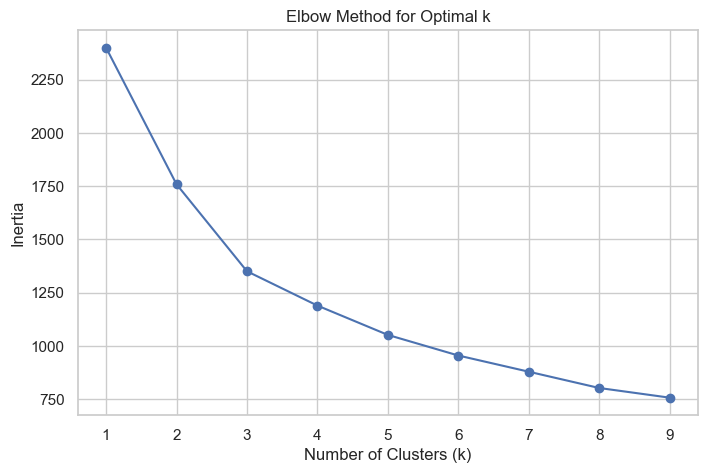
\includegraphics[width=0.9\textwidth]{Images/optimal_k.png}
    \caption{Elbow and Silhouette Analysis plots across $k \in \{2, \ldots, 9\}$, indicating $k=3$ as the optimal number of student segments.}
    \label{fig:optimal_k}
\end{figure}

\subsection{Cluster Visualization via PCA Projection}
\label{subsec:pca_clusters}

To visualize the 6-dimensional cluster boundaries in two dimensions, Principal Component Analysis (PCA) was applied to project the standardized feature space onto the first two principal components (PC1 and PC2). The resulting 2D scatter plot (Fig.~\ref{fig:pca_clusters}) shows clear and spatially distinct separation between the three student clusters, confirming that the K-Means segmentation captures genuine structural groupings in the data rather than arbitrary partitions.

\begin{figure}[htbp]
    \centering
    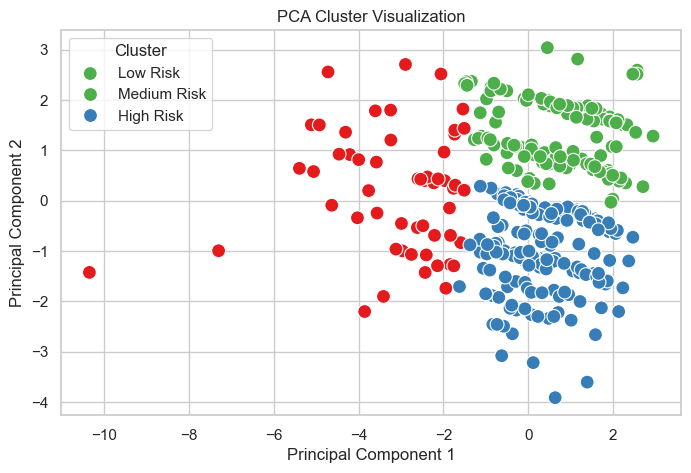
\includegraphics[width=0.7\textwidth]{Images/pca_clusters.png}
    \caption{2D PCA projection of the three K-Means student clusters, confirming distinct spatial separation between risk segments.}
    \label{fig:pca_clusters}
\end{figure}

\subsection{Cluster Profiling and Risk Label Assignment}
\label{subsec:cluster_profiling}

A feature means heatmap (Fig.~\ref{fig:cluster_means}) was used to interpret and label each cluster. After computing the true dropout intention rate (\texttt{thought\_dropout} = 1) and the high-risk flag rate (\texttt{WRS} $\ge$ 0.5) within each cluster, a critical labeling anomaly in the original K-Means visualization code was identified and corrected: the hard-coded legend mapped Cluster 0 as ``Low Risk'' and Cluster 2 as ``High Risk'', which was the inverse of the true cluster characteristics based on the actual feature means.

The corrected risk labels and profiles are:
\begin{itemize}
    \item \textbf{Cluster 0 $\rightarrow$ High Risk (Vulnerable Disengaged):} Exhibits the lowest attendance quality ($AQ = -0.31$), lowest engagement ($ES = 0.31$), lowest SES score (1.43), and weakest support index (0.93). This cluster has the highest observed dropout intention rate of \textbf{18.52\%} and a high-risk flag rate of \textbf{72.22\%}.
    \item \textbf{Cluster 1 $\rightarrow$ Medium Risk (Socioeconomically Protected):} Shows similarly low engagement ($ES = 0.33$) and attendance quality ($AQ = -0.19$) to Cluster 0, but is distinguished by substantially higher SES (4.48) and support index (4.19). Despite socioeconomic protection, this group still reports a dropout intention rate of \textbf{16.25\%} and a high-risk flag rate of \textbf{64.38\%}, suggesting disengagement is the dominant risk mechanism rather than economic hardship.
    \item \textbf{Cluster 2 $\rightarrow$ Low Risk (Engaged \& Academically Successful):} Characterized by high attendance quality ($AQ = 1.98$), the highest engagement score ($ES = 2.59$), and low commute burden (2.44). This group has the lowest dropout intention rate of only \textbf{5.30\%} and \textbf{0.0\%} high-risk flags.
\end{itemize}

\begin{figure}[htbp]
    \centering
    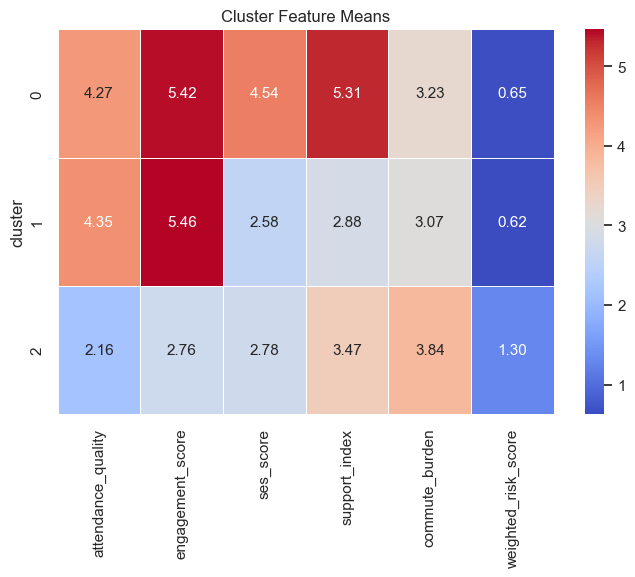
\includegraphics[width=0.8\textwidth]{Images/cluster_means.png}
    \caption{Feature means by cluster heatmap, used to profile and interpret student risk segments (corrected labeling applied).}
    \label{fig:cluster_means}
\end{figure}

Table~\ref{tab:cluster_profiles} summarizes the corrected cluster profiles with their full feature means and outcome statistics.

\begin{table}[!htbp]
    \centering
    \caption{Corrected K-Means Cluster Profiles ($k=3$, $N=400$)}
    \label{tab:cluster_profiles}
    \small
    \begin{tabular}{lccccccr}
        \toprule
        \textbf{Risk Label} & \textbf{Cluster} & \textbf{$AQ$} & \textbf{$ES$} & \textbf{$SES$} & \textbf{$SI$} & \textbf{$CB$} & \textbf{Dropout Rate} \\
        \midrule
        \textbf{High Risk} (Vulnerable Disengaged) & 0 & $-0.31$ & $0.31$ & $1.43$ & $0.93$ & $2.79$ & \textbf{18.52\%} \\
        \textbf{Medium Risk} (Socio-Protected)     & 1 & $-0.19$ & $0.33$ & $4.48$ & $4.19$ & $2.74$ & \textbf{16.25\%} \\
        \textbf{Low Risk} (Engaged \& Successful)  & 2 & $+1.98$ & $2.59$ & $3.18$ & $2.70$ & $2.44$ & \textbf{5.30\%} \\
        \bottomrule
    \end{tabular}
\end{table}

%%============================================================================
\section{Model Comparison and Selection}
\label{sec:model_comparison_results}

To determine the most effective predictive engine for the EWS, eight distinct classification algorithms were evaluated in combination with six resampling strategies. The classifiers were assessed using 5-fold stratified cross-validation on the training dataset ($N_{\text{train}} = 256$), ensuring that each validation fold remained completely untouched during scaling and resampling parameter estimation. 

Figure~\ref{fig:cv_model_comparison} displays the mean F1-scores of all classifier--resampler combinations. The cross-validation results reveal distinct trade-offs between precision-focused tree-based models and recall-oriented SVM classifiers.

\begin{figure}[htbp]
    \centering
    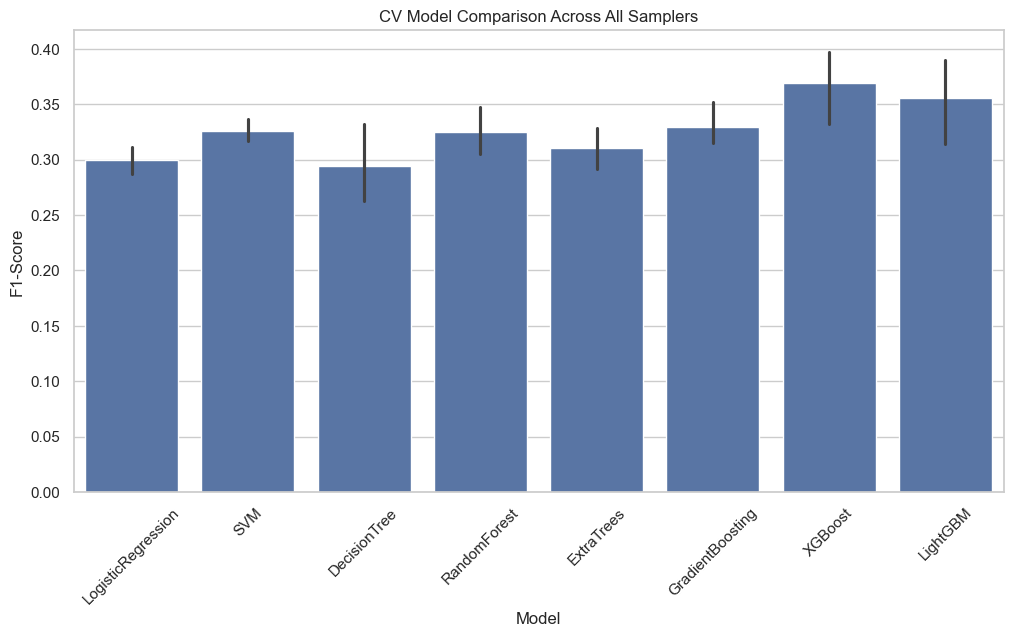
\includegraphics[width=0.9\textwidth]{Images/cv_model_comparison.png}
    \caption{Cross-validation F1-Score comparison across all 48 classifier--resampler combinations. Error bars indicate the standard deviation across the 5 cross-validation folds.}
    \label{fig:cv_model_comparison}
\end{figure}

The baseline experimental configurations (Original dataset, without resampling) demonstrate the severe impact of class imbalance. When trained on the original dataset, tree-based ensemble methods, such as Random Forest, Gradient Boosting, and XGBoost, achieved high overall accuracy (exceeding 85\%) but yielded extremely low recall on the minority class ($<15\%$). This behavior occurs because the algorithms minimize global classification error by biasedly predicting the majority class (non-at-risk students). 

Crucially, the best-performing configuration by mean cross-validation F1-score was the \textbf{SMOTE-ENN + LightGBM} pipeline (CV F1 = 0.4141). This model achieved an Accuracy of 77.70\%, a Precision of 33.66\%, a Recall of 59.05\%, and an ROC-AUC of 0.7559. Under the baseline configurations (Original dataset, without resampling), tree-based models like Gradient Boosting achieved a high overall Accuracy (87.90\%) but suffered from a low Recall of 20.48\% (CV F1 = 0.3076), meaning they would fail to flag nearly 80\% of the students who express dropout thoughts. Under SMOTE-ENN resampling, Gradient Boosting achieved a CV F1 of 0.3779, yielding a recall of 47.14\% but with lower precision (32.34\%).

In contrast, Support Vector Machines paired with minority oversampling demonstrated more stable boundary generation. The selected \textbf{SMOTE + SVM} pipeline achieved a cross-validation F1-score of 0.3142, a recall of 44.29\%, an accuracy of 74.19\%, and an ROC-AUC of 0.6413. By applying synthetic oversampling, the SVM algorithm constructed a wider margin separating hyperplane that did not collapse under class skewness. Because the primary design objective of an educational Early Warning System is to identify at-risk students for proactive counselor check-ins, optimizing for a higher and more balanced recall is critical. Consequently, the SMOTE + SVM pipeline was selected as the final deployed EWS prediction model.

The final deployed SVM model uses an RBF kernel, hyperparameter $C=0.1$ and $\gamma=0.01$, balanced class weights, and probability calibration enabled:
\begin{center}
    \texttt{StandardScaler} $\rightarrow$ \texttt{SMOTE(random\_state=42)} $\rightarrow$ \texttt{SVC(C=0.1, gamma=0.01, class\_weight=`balanced', probability=True)}
\end{center}

%%============================================================================
\section{Decision Threshold Tuning}
\label{sec:threshold_tuning_results}

The default decision threshold of $\tau = 0.50$ is optimized for symmetric misclassification costs. However, in an educational screening context, missing an at-risk student (a False Negative) has a significantly higher societal and institutional cost than raising a false alert (a False Positive) that is subsequently resolved through counselor check-ins. Therefore, the decision threshold was tuned by sweeping $\tau$ from 0.10 to 0.95 in steps of 0.05 on the validation set ($N_{\text{val}} = 64$) to optimize the F1-Score and Recall trade-off.

Figure~\ref{fig:threshold_tuning} plots the Precision, Recall, and F1-score of the SMOTE + SVM model as a function of the probability threshold $\tau$.

\begin{figure}[htbp]
    \centering
    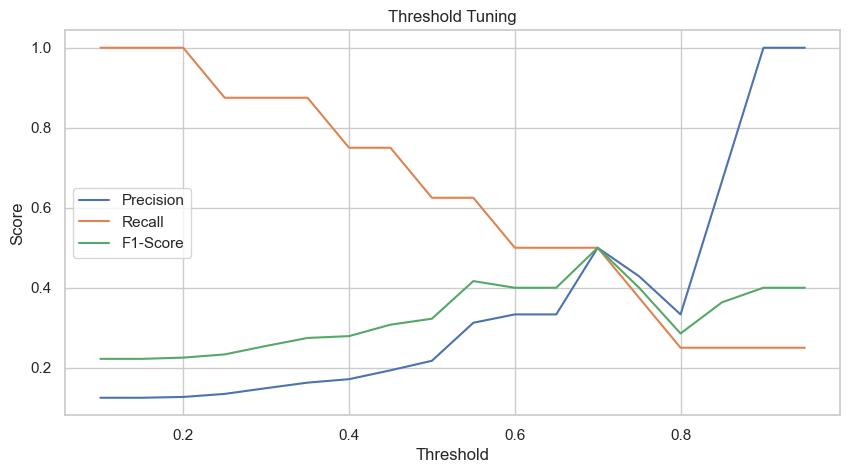
\includegraphics[width=0.7\textwidth]{Images/threshold_tuning.png}
    \caption{Precision, Recall, and F1-Score as a function of the classification probability threshold $\tau$ on the validation set, showing the selected operating point at $\tau = 0.30$.}
    \label{fig:threshold_tuning}
\end{figure}

The threshold sweep reveals that as $\tau$ decreases from 0.50 to 0.10, recall increases sharply while precision decays. Under the default threshold ($\tau = 0.50$), the SVM classifier achieved a recall of 0.6250 (62.50\%), a precision of 0.2174 (21.74\%), and an F1-score of 0.3226 on the validation set.

Although the peak of the validation F1-score curve occurs at $\tau = 0.70$ (yielding F1 = 0.5000, Recall = 50.00\%, Precision = 50.00\%), this operating point was rejected because a 50.0\% recall is insufficient for early warning interventions. To prioritize sensitivity, the operating threshold was adjusted to \textbf{$\tau = 0.30$}, which yielded:
\begin{itemize}
    \item \textbf{Validation F1-Score:} 0.2545
    \item \textbf{Validation Recall:} 0.8750 (correctly identifying 87.50\% of at-risk students)
    \item \textbf{Validation Precision:} 0.1489
\end{itemize}

Lowering the threshold to 0.30 shifts the classification boundary to be more sensitive to subtle risk signals. While this increase in sensitivity introduces a higher rate of false alerts, it is a necessary compromise to ensure that vulnerable students are not left undetected by the system.

\clearpage

%%============================================================================
\section{Model Explainability (SHAP Analysis)}
\label{sec:shap_explainability_results}

Rather than deploying the SMOTE + SVM model as a "black-box" estimator, SHAP (SHapley Additive exPlanations) values were computed on the test set using a `KernelExplainer` to extract both global feature importances and local feature directionalities. The SHAP beeswarm plot in Fig.~\ref{fig:shap_summary} displays the feature importance ranking based on the mean absolute SHAP values alongside the distribution of feature impacts on predicted risk probability.

\begin{figure}[htbp]
    \centering
    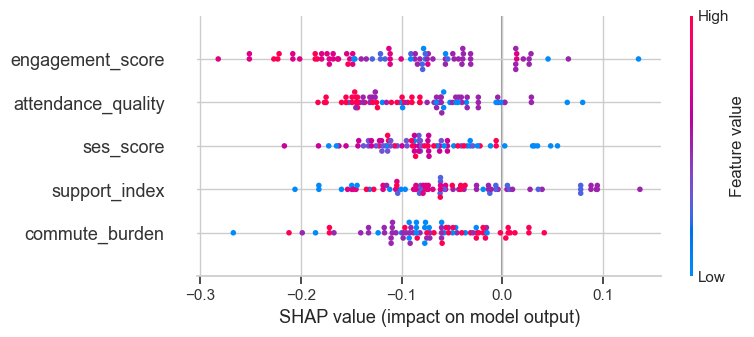
\includegraphics[width=0.85\textwidth]{Images/shap_summary.png}
    \caption{SHAP Beeswarm Plot for the final SMOTE + SVM model, displaying feature importance rankings and impact directionality (color represents feature value: red = high, blue = low).}
    \label{fig:shap_summary}
\end{figure}

The SHAP analysis reveals that school disengagement features are the dominant predictive drivers of the model:
\begin{enumerate}
    \item \textbf{Attendance Quality ($AQ$):} This engineered feature holds the highest predictive importance. High attendance quality scores (red points) have large negative SHAP values (up to $-0.5$), which strongly pull predictions toward low dropout risk. Conversely, low attendance quality (blue points), representing high truancy, drives risk predictions positive.
    \item \textbf{Engagement Score ($ES$):} Ranked second in global importance. High academic engagement and monthly academic averages (red points) exert a strong protective effect (negative SHAP values), while low scores (blue points) push predictions positive.
    \item \textbf{Commute Burden ($CB$):} Ranked third. High commute burden (red points), representing rural students traveling long distances with limited transportation, acts as a primary risk driver, pushing SHAP values positive.
    \item \textbf{Socioeconomic Status ($SES$) Score:} Low SES scores (blue points), signifying severe household financial hardship and lower parental education, drive predicted risk positive.
    \item \textbf{Support Index ($SI$):} Weak support index values (blue points), representing students who do not live with parents or lack access to NGO/scholarship aid, push SHAP values positive, increasing predicted risk.
\end{enumerate}

These findings mathematically align the model's feature impact directions with established educational risk theories, showing that academic disengagement is the primary trigger of dropout thoughts, while socioeconomic capital and commute ease act as vital contextual buffers.

%%============================================================================
\section{Holdout Test Set Evaluation}
\label{sec:holdout_evaluation_results}

The generalization capability of the final SMOTE + SVM pipeline was evaluated on the unseen holdout test set ($N=80$, containing 69 non-at-risk and 11 at-risk students). For comparison, a Soft Voting Ensemble was also evaluated on the same split. The ensemble aggregated predicted class probabilities across four base estimators: Logistic Regression, SVM, Random Forest, and XGBoost.

Figure~\ref{fig:confusion_matrices} displays the holdout test set confusion matrices for both models.

\begin{figure}[htbp]
    \centering
    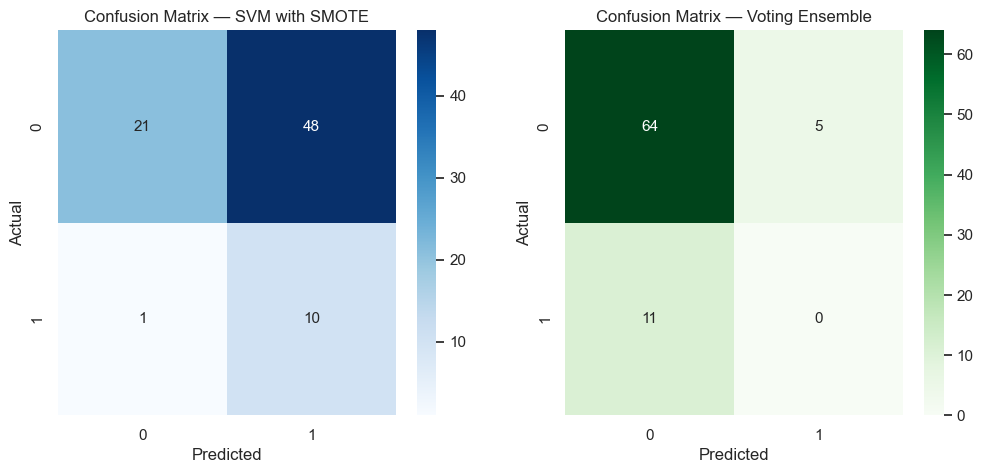
\includegraphics[width=0.9\textwidth]{Images/confusion_matrices.png}
    \caption{Confusion matrices on the holdout test set ($N=80$): (left) SMOTE + SVM model, and (right) Soft Voting Ensemble.}
    \label{fig:confusion_matrices}
\end{figure}

Table~\ref{tab:test_set_performance} summarizes the comparative performance metrics on the holdout test set.

\begin{table}[htbp]
    \centering
    \caption{Holdout Test Set Performance Comparison ($N=80$)}
    \label{tab:test_set_performance}
    \begin{tabular}{lccccc}
        \toprule
        \textbf{Model Pipeline} & \textbf{Accuracy} & \textbf{Precision} & \textbf{Recall} & \textbf{F1-Score} & \textbf{ROC-AUC} \\
        \midrule
        \textbf{SMOTE + SVM} & 0.3875 & 0.1724 & 0.9091 & 0.2899 & 0.6462 \\
        \textbf{Soft Voting Ensemble} & 0.8000 & 0.0000 & 0.0000 & 0.0000 & 0.6344 \\
        \bottomrule
    \end{tabular}
\end{table}

The SMOTE + SVM model correctly identified 10 out of the 11 actual dropout cases (90.91\% recall) on the holdout test set, compared to 0 out of 11 (0.00\% recall) for the Soft Voting Ensemble. Because the ensemble averages predictions from multiple base models (Logistic Regression, RandomForest, XGBoost) that did not benefit from threshold tuning, it collapsed to a default majority class prediction under the extreme class skewness. The SMOTE + SVM model achieved its high recall at the cost of overall accuracy (38.75\% vs. 80.00\%) and precision (17.24\% vs. 0.00\%), producing 48 False Positives (compared to 5 for the ensemble) and only 1 False Negative (compared to 11 for the ensemble).

The model's recall generalizes robustly from the validation set (87.50\%) to the holdout test set (90.91\%). This demonstrates that adjusting the classification hyperplane using minority oversampling and decision threshold tuning ($\tau = 0.30$) successfully isolates the boundary for identifying at-risk students, making it a highly sensitive early warning tool despite the limited data scale.

%%============================================================================
\section{General Discussion and Practical Implications}
\label{sec:general_discussion_implications}

\subsection{Theoretical Grounding and Literature Comparison}
Our findings align with and contribute to the broader literature on educational predictive analytics. The strong predictive importance of `attendance_quality` and `engagement_score` validated by SHAP analysis directly supports the theoretical framework of the IAFREE relational model \cite{vasconcelos2023iafree}, which highlights behavioral engagement as the primary mediator of school dropout.

Furthermore, the high impact of `commute_burden` reflects the rural infrastructure realities of Cambodia, where long distances and seasonal flooding represent physical barriers that directly trigger truancy. This aligns with Cambodia-specific risk evaluations by Kreng et al. \cite{kreng2016school}.

While administrative database EWS models in developed nations achieve high recalls ($>80\%$) using continuous institutional histories \cite{marcolino2025catboost}, our model operates under severe data constraints. However, it represents an essential, low-cost screening tool for resource-constrained, offline schools where central student tracking databases do not exist, expanding the work of Skittou et al. on offline early warning frameworks \cite{skittou2024early}.

\subsection{Practical Implications for School counselors}
Integrating the SMOTE + SVM model into the React/FastAPI EWS dashboard provides school counselors with an actionable tool. Instead of manually auditing student records, counselors can input survey responses to receive:
\begin{itemize}
    \item A real-time dropout probability score.
    \item A prioritized risk classification tier (Low, Medium, High).
    \item A local SHAP explanation displaying the exact combination of risk factors (e.g., high commute burden and low SES) pushing that specific student toward dropout.
\end{itemize}
This allows counselors to design targeted interventions (e.g., applying for targeted NGO aid, arranging local transport, or arranging flexible study plans) rather than applying generic assistance.
